\chapter{Clients projects}

During the development of the Site Builder I also worked on side projects for Hindsite's clients.
These projects need a very different way to work than the Site Builder. I had to adapt my code to the existing one, 
get the work done in the fastest way possible, work under very short deadline.

I had to deal with new challenges. Before that I was not directly involved with clients. With these projects 


\section{Sencore}

The Sencore website was designed and developed before I began my internship. Since the main developer on this project finished its internship, I was in charge of the maintenance and adding the new features. One of these features was to implement in a very short time a video player for movies hosted on the site's ftp server.

I used JQuery technology to show a popup over the current opened page. It allows to scale and position the video player exactly on the middle of the page. 

\begin{figure}[!ht]
\centering
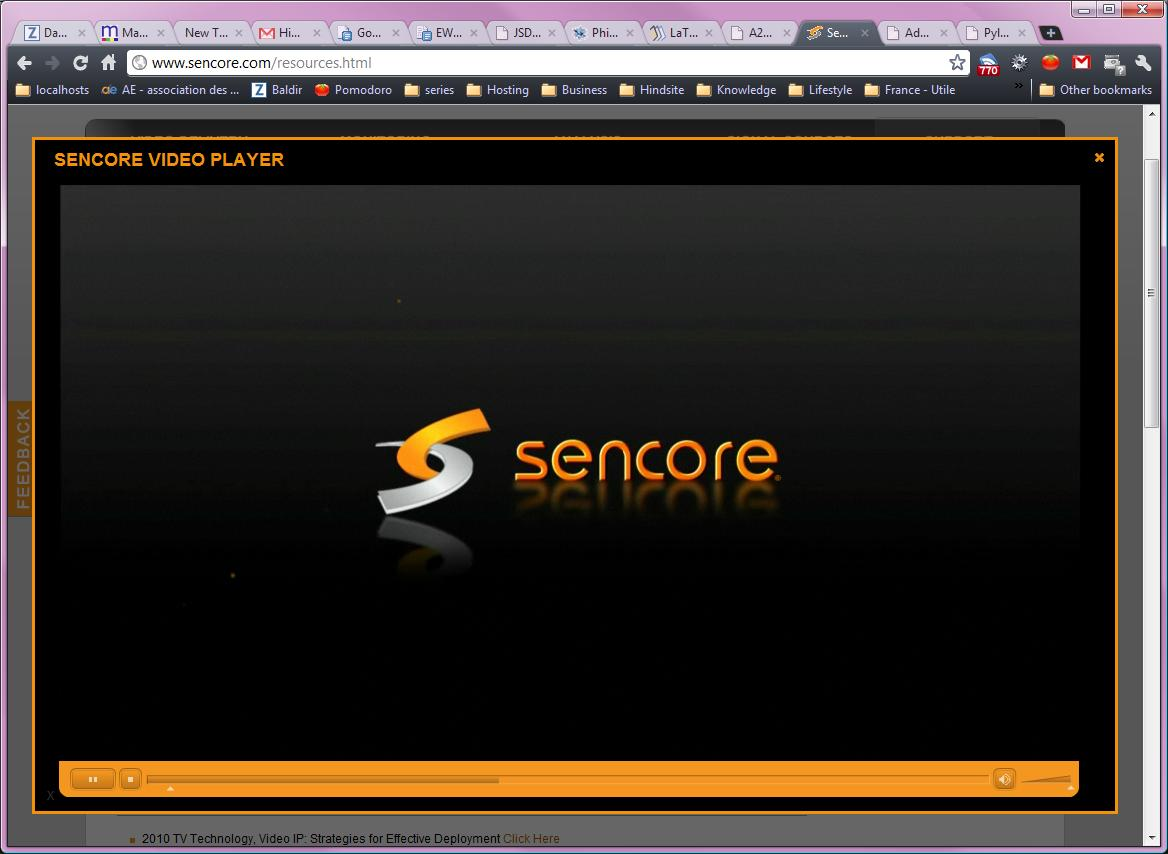
\includegraphics[width=.55\textwidth]{img/sencore_video.jpg}
\caption{Sencore video player}
\label{figure:sencore_video}
\end{figure}

\section{A2LA}

A2LA as "The American Association for Laboratory Accreditation" proposes registration for their different courses. 
I had to create a new Form payment for the annual forum of A2LA. This page has to take some values from a form hosted in another domain. 

This page also have to be secure and be able to send mails either to a2la executives and payment confirmation to the client.
The secured payment is provided by Authorize.net through its API. I also had to implement additional securities into my pages so that nobody can do illicit actions.

I implemented a section in the already existing administration area to provide summary of the operations that have been done with the forms.

\begin{figure}[!hb]
\centering
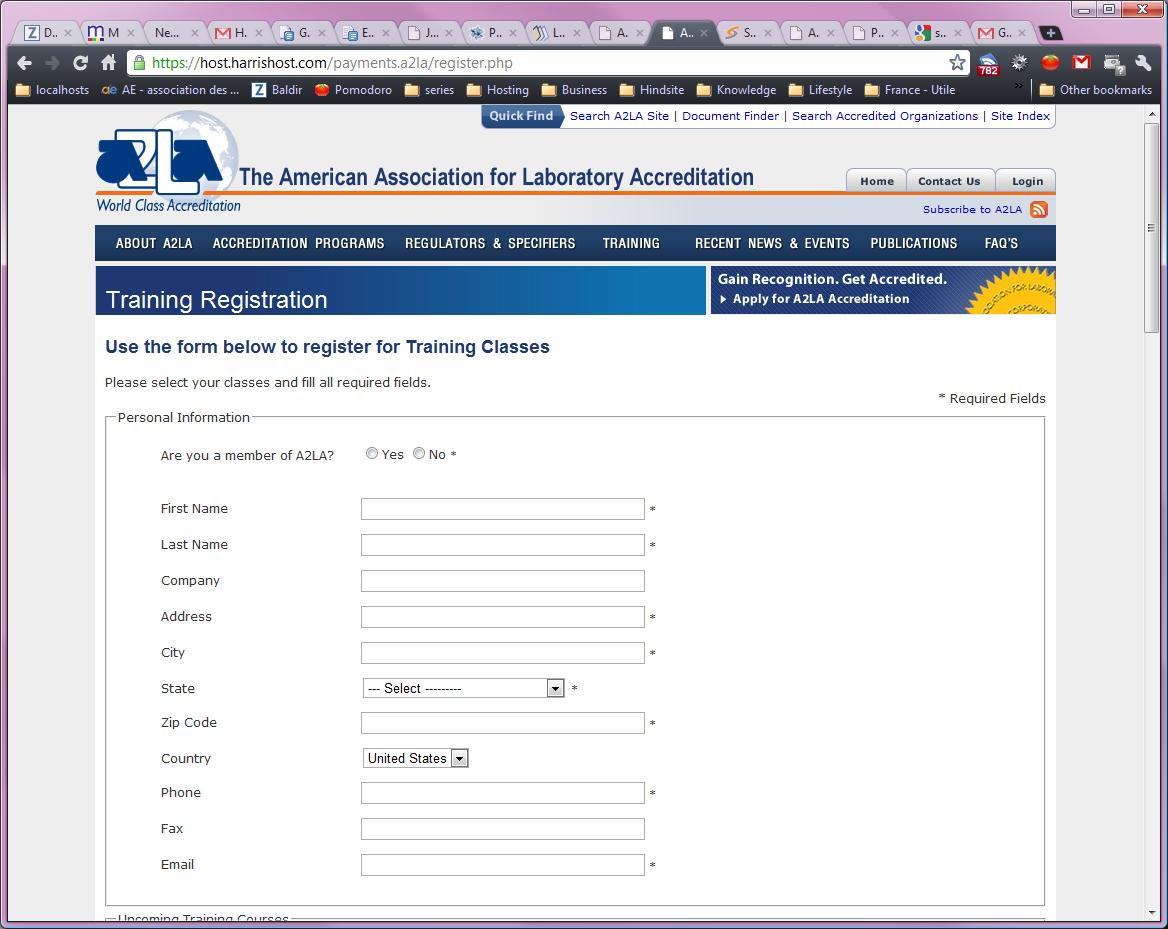
\includegraphics[width=.55\textwidth]{img/a2la.jpg}
\caption{A2LA Forum registration form}
\label{figure:a2la_reg}
\end{figure}


\section{Advanced Centrifugals ltd}
Advanced Centrifugals is an industry leader in centrifugally cast heat and corrosion resistant alloy tubes. 
The web site of the company ( \url{http://advancedcentrifugalsltd.com}) was already designed by Hindsite. 

\begin{figure}[!h]
\centering
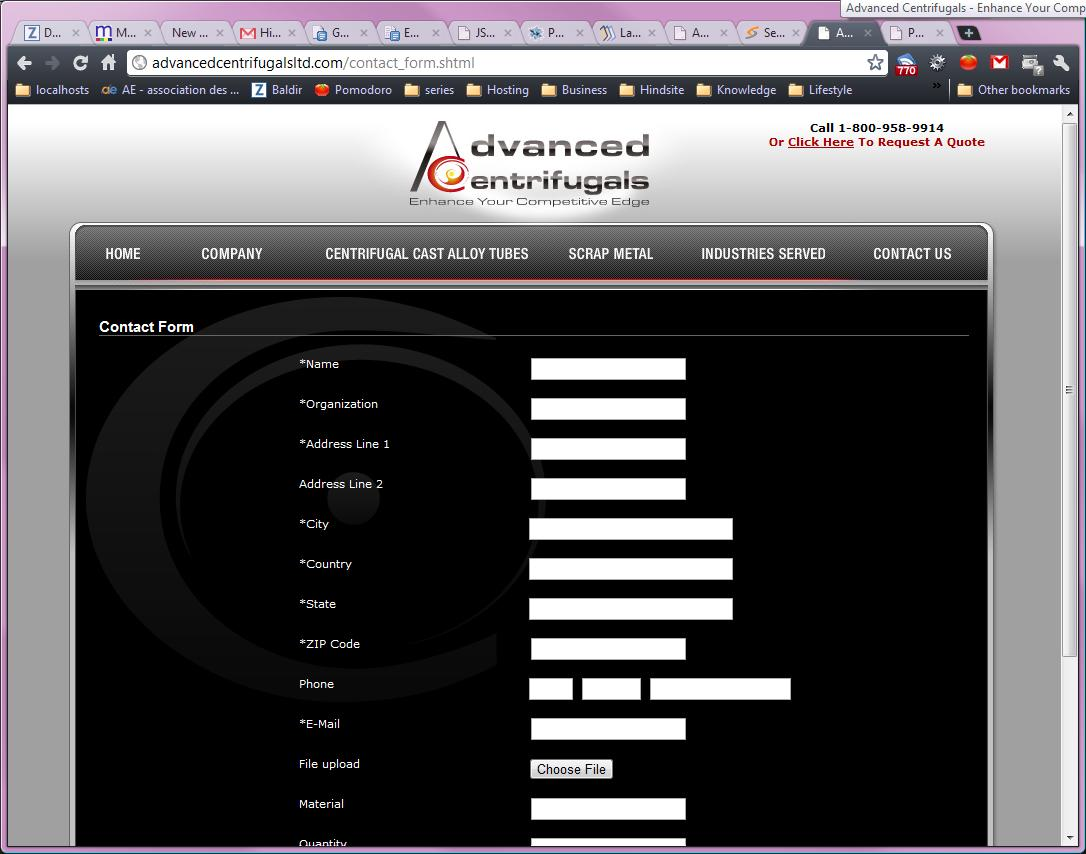
\includegraphics[width=.55\textwidth]{img/adv_1.jpg}
\caption{Advanced Centrifugals contact form}
\label{figure:adv_1}
\end{figure}

I had to adapt a contact form that also send mail to advanced centrifugals and store information in a database.
The information is accessible in an administration panel.

\begin{figure}[!h]
\centering
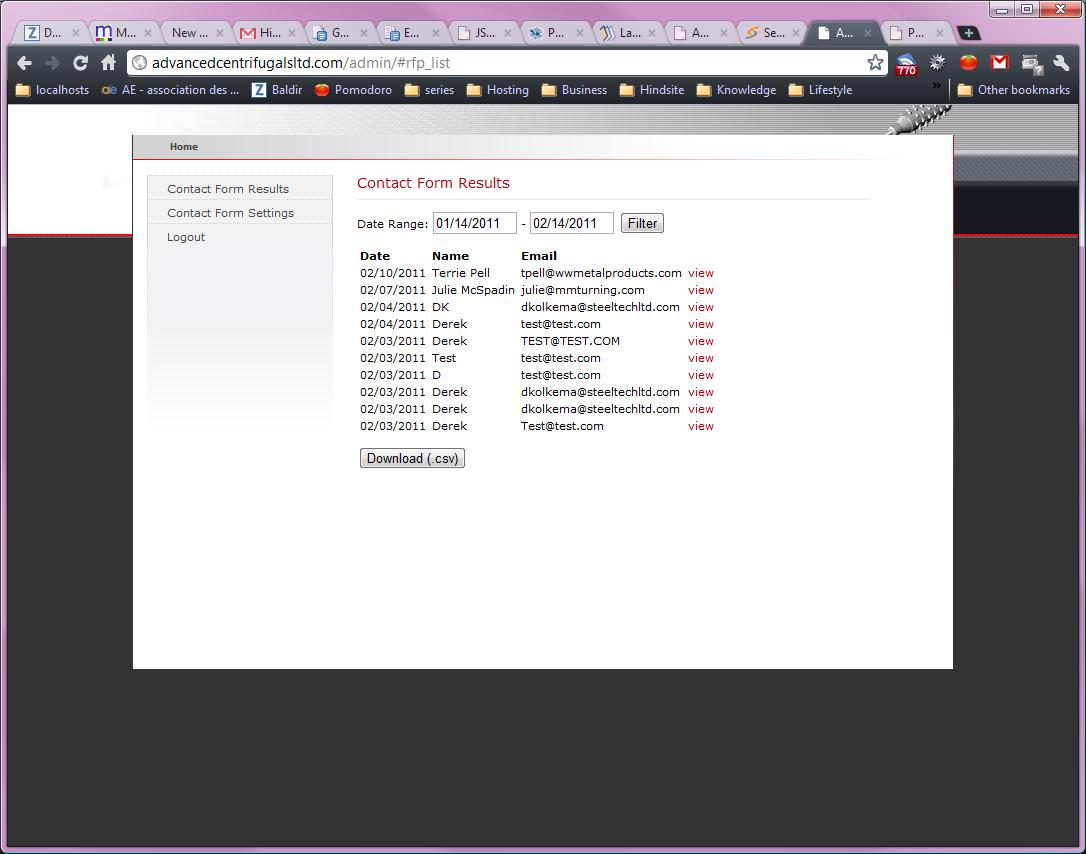
\includegraphics[width=.55\textwidth]{img/adv_2.jpg}
\caption{Advanced Centrifugals Administration area}
\label{figure:adv_2}
\end{figure}

\section{Pylon}

Pylon is a manufacturer and distributor of wiper blades. The web site of this company is pretty old and the code behind have got layer over layer of technology. Originally written in PHP 4, it still uses deprecated functions and libraries to work. 
I had to dig deeply into the code to understand how to simply add and modify a page, how to customize the administration panel and how to manipulate data in order not to add more complexity.

\begin{figure}[!h]
\centering
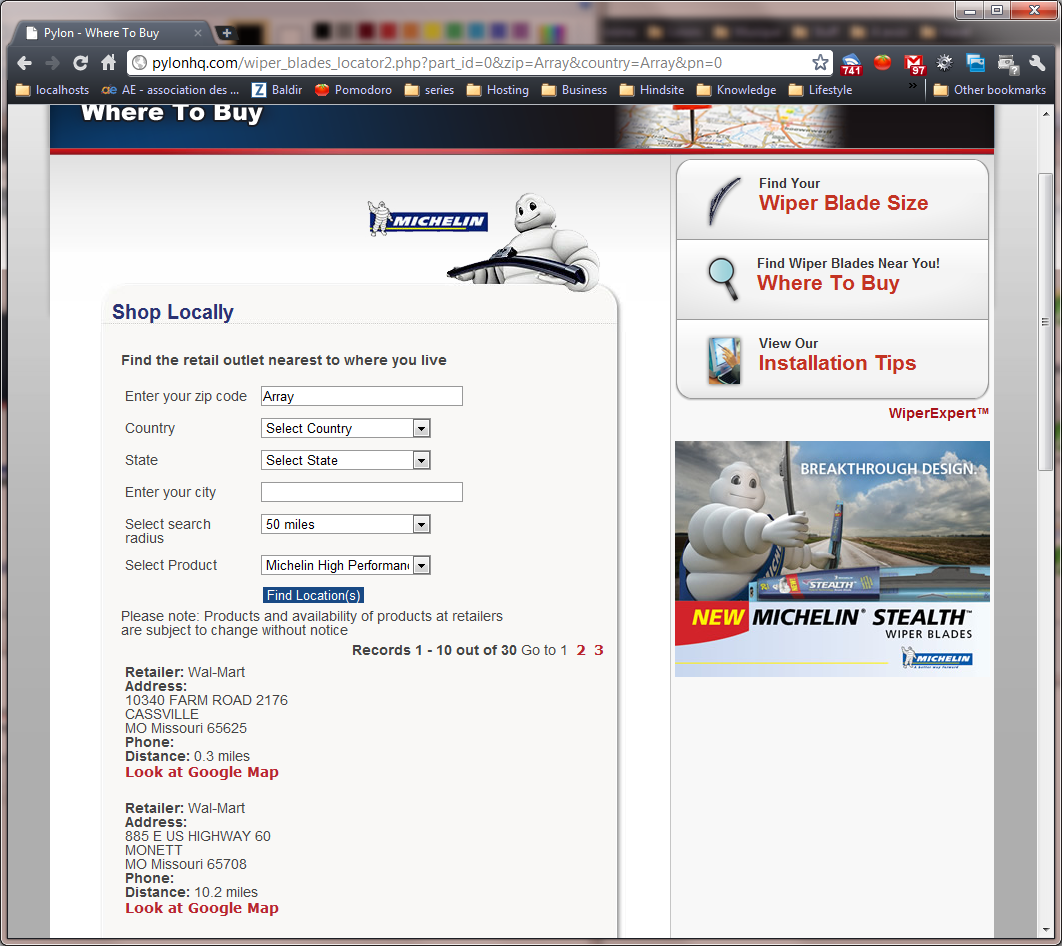
\includegraphics[width=.55\textwidth]{img/pylon_v.png}
\caption{Pylon shop finder}
\label{figure:pyl_shop}
\end{figure}
 
The main tasks I was asked on this project was to upgrade the form to search where to buy a product by allowing to filter by product (see figure \ref{figure:pyl_shop} p. \pageref{figure:pyl_shop}). Another was to enhance existing form that allowed to know what wiper blade correspond to your car by adding geographic information and a link to the previous form (see figure \ref{figure:pyl_vehicle} p. \pageref{figure:pyl_vehicle}).

\begin{figure}[!h]
\centering
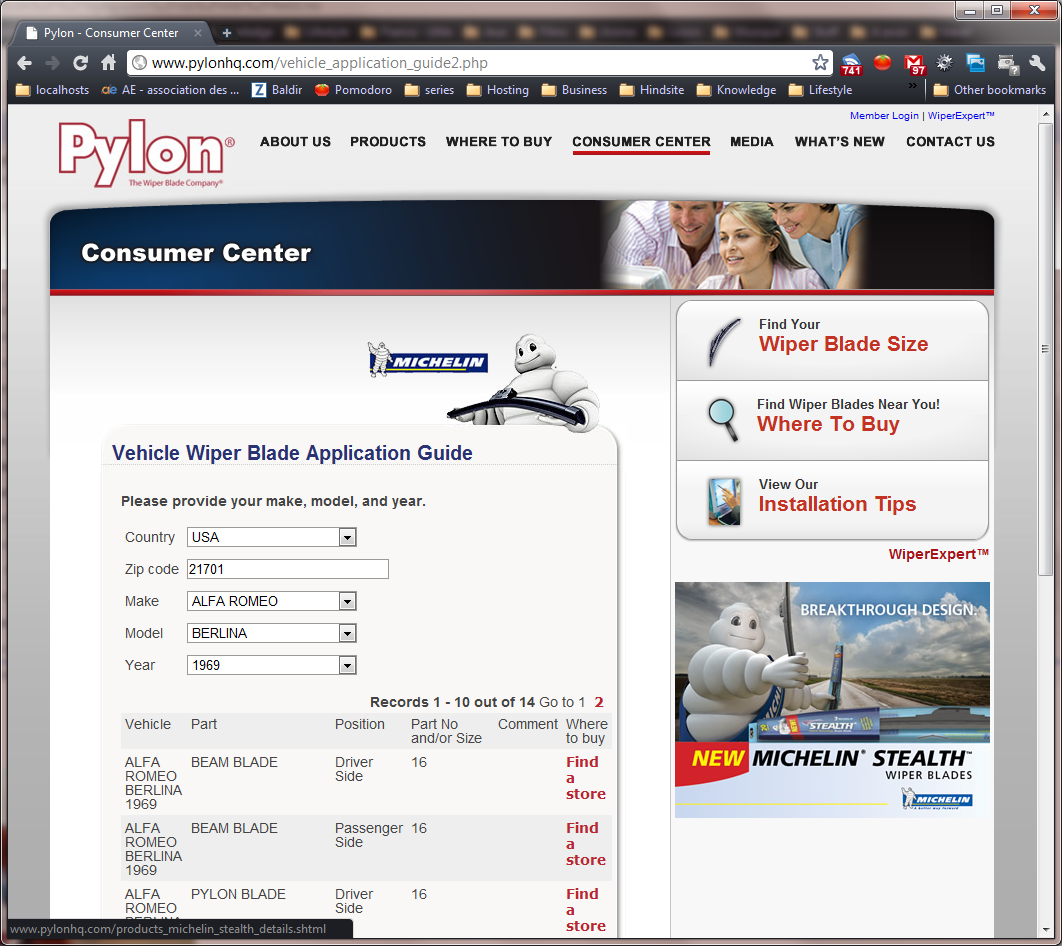
\includegraphics[width=.55\textwidth]{img/pylon_vehicule.png}
\caption{Pylon vehicle part finder}
\label{figure:pyl_vehicle}
\end{figure}

By the administration panel i had to develop a data import feature using CSV files and populating the database. I also added an export feature to load the data from the database and create a CSV file.
